\section{Oblikovanje završnog rada}

\subsection{Odabir uređivača teksta}

Za pisanje rada možete koristiti bilo koji program za obradu teksta (engl.~\textit{word processor}) kao što su Microsoft Office, LibreOffice i Google Documents ili slovoslagarski program npr.~\LaTeX. Bez obzira koji se alati za oblikovanje teksta koriste, završni rad mora biti korektno formatiran. U slučaju da se koristi neki od WYSWYG (\textit{what you see is what you get}) uređivača teksta preporuka je da se unaprijed definira 
stil dokumenta. Dakle, unaprijed se definiraju veličine naslova, podnaslova, fontovi i slično. Važno je da određeni stil prati cijeli završni rad. 


U slučaju da student želi koristiti \LaTeX, može dobiti predložak ovog dokumenta za pomoć pri izradi rada.

\subsection{Osnovne postavke oblikovanja teksta}
Prilikom izrade tekstualnog dijela završnog rada treba pratiti sljedeće upute:
\begin{itemize}
 \item Format papira A4.
 \item Font Times New Roman ili neki slični, veličina 12pt.
 \item Margine:
 \begin{itemize}
  \item gornji rub: 25 mm
  \item donji rub: 30 mm
  \item unutarnji rub (lijevi): 30 mm
  \item vanjski rub (desni): 25 mm
 \end{itemize}
 \item Obostrano poravnanje.
 \item Prored teksta 1.5 (engl.~\textit{line spacing}).
 \item Početak odlomka mora biti uvučen. Redak se uvlači na početku svakog odlomka. Između odlomaka treba biti veći razmak.
 
 \end{itemize}
%\subsubsection*{Numeriranje}
Naslovnica nije numerirana. Sadržaj je numeriran rimskim brojevima. Sve ostale stranice u završnom radu trebaju biti numerirane arapskim brojevima unutar donje margine. 

\subsection{Struktura završnog rada}
\textbf{Naslovna} i \textbf{prva stranica} završnog rada definirane su Pravilnikom za izradu i obranu završnog rada. Njih slijedi \textbf{sadržaj} koji treba biti generiran iz naslova poglavlja i potpoglavlja.

Slijedi \textbf{sažetak} u kojem u nekoliko rečenica treba navesti što je cilj završnog rada i kako se do njega došlo (što je analizirano, razvijeno, izrađeno). Na kraju sažetka mogu se navesti ključne riječi koje su važne za rad. Na istoj stranici ispod sažetka treba napisati i sažetak na engleskom jeziku (engl.~\textit{summary}). Na početku sažetka na engleskom jeziku treba podebljanim tekstom napisati naziv teme na engleskom jeziku. Kao i za sažetak na hrvatskom treba prevesti ključne riječi na engleski jezik (engl.~\textit{keywords}).

Potom se u \textbf{uvodu} opisuje problem, motivacija za rad (zbog čega je ponuđeno rješenje uopće potrebno) i način na koji ste rješavali problem te glavni doprinosi. Na kraju uvoda sažeto se opisuju ostala poglavlja rada.

\textbf{Glavni dio} treba suvislo podijeliti na više poglavlja. U pravilu se počne sa specifikacijom te poglavljem o metodama i alatima koji su korišteni (opis metoda, opis alata, primjeri tipične uporabe i sl.). U idućem poglavlju opisuje se sam rad i doprinosi. Na primjer, detaljno se opisuje metoda ili sustav koji je razvijen prilikom izrade završnog rada te detaljan opis implementacije. Ako se razvijaju samo dijelovi sustava, tj.~neke komponente sustava, mogu se dati primjeri upotrebe. U sljedećem poglavlju može se detaljno opisati aplikaciju odnosno praktični rad. Ako sustav ima korisničko sučelje slikama se prikazuju snimke zaslona pri tipičnoj uporabi aplikacije. Ako se u radu razvija novu metodu, ovo poglavlje može biti namijenjeno njenoj eksperimentalnoj evaluaciji i raspravi o eksperimentalnim rezultatima.

Na kraju se piše \textbf{zaključak}. On može početi s jednostavnim opisom što je u radu napravljeno i koji su glavni doprinosi rada. Nakon toga može se napisati nekoliko rečenica u kojima se opisuje zašto je napravljeno uopće važno, kakva je moguća upotreba i što se predlože kako bi se napravljeno poboljšalo u skladu s postavljenim ciljevima. Ako se razvijena aplikacija već koristi mogu se opisati povratne informacije korisnika.

U \textbf{literaturi} se navode izvori po redoslijedu pojavljivanja u tekstu. Navode se samo oni izvore na koje se u radu poziva.

Na kraju rada treba dodati i \textbf{izjava o autentičnosti završnog rada} koja se nalazi na našim internetskim stranicama.

\subsection{Slike, tablice i programski k\^od}
U završni rad uključuju se slikovni prikazi (grafovi, sheme, ilustracije, snimke zaslona i sl.) koji povećavaju razumljivost i čitljivost rada. Slike moraju biti numerirane u tekstu te imati odgovarajući naziv (engl.~\textit{caption}) neposredno ispod slike. U rad umetnite slike otprilike uz dio teksta iz kojeg se pozivate na njih. Svaka slika treba biti referirana na barem jednom mjestu u tekstu. Slike centrirajte kao i njihov naziv. Primjerice, na slici~\ref{fig:xfce} je prikazan jedan od bezbroj mogućih izgleda radne okoline.
\\[\intextsep]
\begin{minipage}{\linewidth}
\centering%
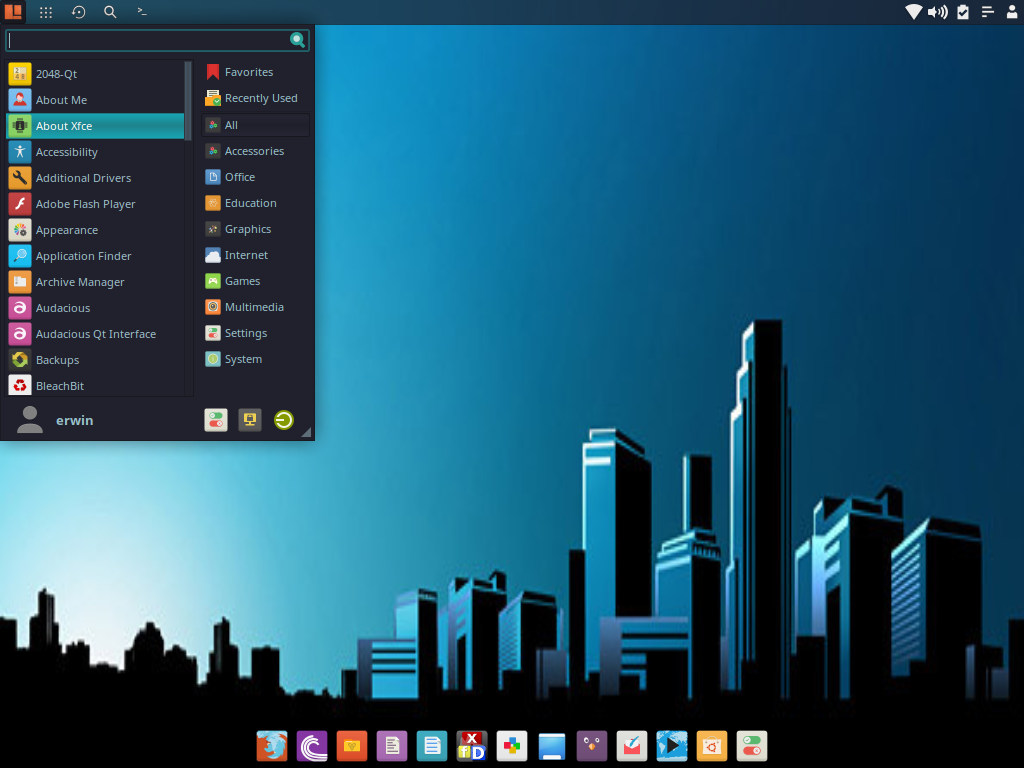
\includegraphics[width=0.4\linewidth,clip=]{slike/xfce.png}
\figcaption{Primjer radne okoline Xfce}%
\label{fig:xfce}%
\end{minipage}
\\[\intextsep]
Rezultati eksperimenata mogu se prikazati u tablicama koje moraju biti numerirane i imati naziv kao i slike. Naziv i opis tablice nalazi se neposredno iznad tablice. Tablica mora biti referirana na barem jednom mjestu u tekstu, kao u sljedećem primjeru: U tablici~\ref{fig:ioesc} opisane su najčešće \textit{escape} sekvence.
\begin{longtable}{l l }
\caption{Escape sekvence}\label{fig:ioesc}
\endfirsthead
\endhead
\hline
oznaka&opis \\
\hline
\lstinline!\n!&novi red \\
\lstinline!\t!&horizontalni tab\\
\lstinline!\v!&vertikalni tab\\
\lstinline!\'!&apostrof \\
\lstinline!\"!&dvostruki navodnik \\
\lstinline!\\!&\textit{backslash} znak \\
\lstinline!\?!&upitnik\\
\hline
\end{longtable}

Programski k\^od se piše fontom u kojem su sva slova jednake širine (engl.~\textit{monospace}). Primjer takvog fonta je \texttt{courier}. %Listu slobodnih \textit{monospace} fontova možete naći na stranicama \url{http://www.fontsquirrel.com/fonts/list/classification/monospaced}. 
Veličina slova treba biti nešto manja nego u običnom tekstu. Primjer k\^oda je dan u ispisu~\ref{program}.
%
%\begin{lstlisting}
%#! /bin/bash
%# skripta za prebacivanje "layout-a" tipkovnice
%setxkbmap $1
%echo Prebacili ste na $1 tipkovnicu.
%\end{lstlisting}
%\caption{Skripta za mijenjanje položaja tipkovnice}
%\label{fig:program}
%\end{figure}

\begin{lstlisting}[caption={Skripta za mijenjanje rasporeda tipki tipkovnice}, label=program]
#! /bin/bash
# skripta za mijenjanje "layout-a" tipkovnice
setxkbmap $1
echo Prebacili ste na $1 tipkovnicu.
\end{lstlisting}

U tekstu prilikom navođenja naziva varijabli, memorijskih lokacija, putanja i naziva direktorija i datoteka, naziva metoda i funkcija koristi se neki iz \texttt{monospace} obitelji fontova.
\subsection{Pravopis i gramatika}

Studenti su obavezni predati pravopisno i gramatički ispravan rad. Završni radovi koji nisu ispravno napisani neće biti mentorirani. Provjera ispravnosti riječi može se obaviti putem stranice \href{http://hjp.znanje.hr/}{hrvatskog jezičnog portala}. Pravila hrvatskog pravopisa mogu se naći na stranicama \href{www.pravopis.hr}{www.pravopis.hr}. Među pravilima treba obratiti pažnju na pisanje tuđica, koje su uobičajene u pisanju radova iz područja računarstva. Osim toga, obavezna je i provjera teksta alatima za jezičnu provjeru (engl.~\textit{spell checker}) hrvatskog jezika. Ako ga nemate, na stranicama \url{https://hacheck.tel.fer.hr/} nalazi se online alat.
\subsection{Kratice}

Prilikom prvog pojavljivanja, kratice u tekstu se opisuju, a u daljnjem tekstu se koriste bez ponovnog opisa. 

\subsection{Strane riječi}
U završnom radu koristi se hrvatski jezik kada za određenu riječ postoji hrvatski prijevod. Ukoliko korištenje takve hrvatske riječi nije 
uobičajeno u praksi ili autori rada ne 
poznaju odgovarajuću hrvatsku riječ, ostavlja se strana riječ napisana \textit{u kurzivu}.

Kada se prvi put uvodi pojam na hrvatskom jeziku, potrebno je u zagradama navesti i originalnu riječ. Npr. jezgra (engl.~\textit{kernel}) operativnog sustava.  

\subsection{Stil}
Završni rad se piše u neutralnom stilu i bezlično npr. "ispitivanje je pokazalo...". 
Preporučljivo je izbjegavati prvo lice jednine i prvo lice množine osim na mjestima gdje se ističe osobna odluka između više mogućnosti. 


\subsection{Popis literature}
Navode koji su preuzeti iz vanjskih izvora potrebno je potkrijepiti referencom (broj u uglatim zagradama po redoslijedu pojavljivanja). Broj se odnosi na izvor podataka naveden u popisu literature. Fusnote na dnu stranice treba izbjegavati jer nisu uobičajeni oblik citiranja za tehničke radove. Internetski izvori moraju imati u zagradama na kraju datum kad je stranica zadnji put posjećena. Reference treba oblikovati prema IEEE stilu pisanja radova~\cite{IEEE}.

U popisu literature treba navesti literaturu koja se koristila za izradu rada te popis web stranica. Izvore navedite po redoslijedu pojavljivanja u tekstu. Navedite samo one izvore na koje se u radu pozivate. Popisi trebaju biti 
grupirani na način da se najprije navede popis literature, a zatim popis web stranica s datumom zadnjeg pristupanja stranici. Literatura se navodi kako slijedi:
\begin{enumerate}
\item 
Prezime autora, inicijal imena: Naslov knjige, izdavač, mjesto i godina izdavanja
\item Prezime autora, inicijal imena: Naslov rada, naziv skupa, časopisa ili zbornika radova,
mjesto i godina objavljivanja
\item Prezime autora, inicijal imena: Naslov rada, web stranica objavljivanja
\end{enumerate}

\subsection{Plagiranje}

Citiranje je doslovno preuzimanje dijelova drugog rada. Citira se u navodnicima uz referencu na izvor podataka. 
Svako preuzimanje dijelova teksta koji nije ispravno citiran smatra se plagijatom i nije dopušteno u izradi završnog rada.

Parafraziranje je vlastitim riječima opisan dio drugog rada, u kojem slučaju je potrebno navesti izvor 
parafraziranog teksta. Doslovno prevođenje sa stranog jezika smatra se plagijatom. Ukoliko student pošalje rad za koji mentor utvrdi da je plagiran u bilo kojem dijelu teksta, mentor neće mentorirati ni ispravljati ostatak završnog rada.

\subsection{Imenovanje dokumenta}
Završni rad predaje se u pdf formatu. Ukoliko se tijekom izrade šalje na provjeru mentoru, svaka nova verzija dokumenta treba biti 
ispravno numerirana kako bi se iz imena 
dokumenta lako moglo odrediti da li je dokument noviji od prethodno poslanih. Npr.~pet dokumenata koji se šalju na čitanje mogu biti 
imenovani na sljedeći način:
\\
\texttt{prezime\_zavrsni\_1.0.pdf}\\
\texttt{prezime\_zavrsni\_1.1.pdf}\\
\texttt{prezime\_zavrsni\_1.2.pdf}\\
\texttt{prezime\_zavrsni\_1.3.pdf}\\
\texttt{prezime\_zavrsni\_2.0.pdf}\\
Nula na kraju imena (1.0, 2.0 itd) označava verzije sa važnim izmjenama, dok se verzije sa manjim izmjenama označavaju ostalim brojevima (1.1, 1.2, 2.1 itd). 

Osim navedene mogućnosti numeriranja, postoji mogućnost da pri izradi završni rada koristi neki do sustava za kontrolu verzija (\textit{git, subversion, cvs}). Odabir takve mogućnosti je poželjan.

\subsection{Jezični savjeti}
\begin{itemize}
\item 
Završni rad je napisan na hrvatskom jeziku. Možda će uskoro biti moguće pisati i na nekom od svjetskih jezika, ali za sada je moguće jedino na hrvatskom jeziku.
\item Završni rad mora biti napisan u skladu sa standardom i pravilima jezika. Preporučujemo da pismeni dio rada pregleda lektor ili ga pregledajte na neki drugi način. Stručni rad nije literalni tekst pa za njega vrijede drukčija pravila.
\item Stručni tekst mora biti jednoznačan, stoga pišite u kratkim, jednostavnim i jasnim rečenicama.
\item Pišite u neutralnom stilu u pasivu, npr.: „razvijen je“, „napravljeno je“, „napisano je“ i sl. Izbjegavajte prvo lice jednine i množine osim na mjestima na kojima želite istaknuti svoju osobnu odluku između više mogućnosti. 
\item Za pojedini pojam ili objekt u cijelom radu koristite istu oznaku ili ime.
\item Ako uvodite nove pojmove pazite da su jednoznačno i pravilno definirani.
\item Koristite važeću stručnu terminologiju (ne server nego poslužitelj, ne hardware nego strojna oprema ili eventualno hardver, ne elektronska pošta nego elektronička pošta, ne računar nego računalo, ne router ili ruter nego usmjernik, ne Internet nego internet). Postoji mnogo internetskih izvora na koja vas može uputiti vaš mentor.
S pisanjem stručnih riječi se razvija i hrvatska stručna terminologija. Tamo gdje je smisleno u suradnji s mentorom predložite hrvatski prijevod za stručne izraze koji još nemaju prijevoda.
Posebnu pozornost posvetite prijevodima s engleskog jezika. Pri tomu pazite na pravila hrvatskog jezika. Samostalni pridjevi su na hrvatskom jeziku na desnoj strani imenice ili predmeta (SQL query je upit SQL, x-axis je os x, Laravel framework je razvojni okvir Laravel, Linux operation system je operativni sustav Linux i sl.). Obratni redoslijed je pogrešan: SQL upit, x os, Laravel razvojni okvir ili Linux operativni sustav.

\item Iza znaka interpunkcije (točka, zarez, upitnik, uskličnik i slično) stavlja se razmak. Razmak dolazi i prije otvorene zagrade, ali ne i nakon otvorene zagrade i prije zatvaranja zagrade. 
Nakon zagrade ponovo se stavlja razmak.

\item Između broja i znaka za mjernu jedinicu piše se razmak.

\item Riječ k\^od piše se s akcentom.                               
\end{itemize}
